\chapter{Conclusion, Discussion and Future Work\label{chap:discussion}}
In this chapter, I conclude the work conducted in this paper, reflect on the results and suggest the next steps for the designed framework. I also overview my achievements, slowdowns and difficulties found.

\section{Summary}
In this dissertation, I have introduced a novel method of authenticating clients connecting to arbitrary MQTT Brokers through a middleware framework storing persistent information on Ethereum blockchain, allowing for higher transparency and availability. I have started by providing a motivation for the project, bringing up that standard MQTT protocol offers only limited authentication methods, with no option to log audit trails. Recent legislature requiring data administrators to adhere to a specific set of rules dictating how the data should be stored, maintained and erased if requested was also discussed.

As the project involved a lot of sophisticated software such as MQTT or Blockchain, a thorough background chapter was included in order to allow the reader to better understand the concepts and decisions taken throughout this thesis. An overview of related papers has also been included to make sure that my efforts were not duplicating any similar research.

Before discussing the design of the framework, I explored and listed requirements for the project formulated as user stories, scenarios and list of functional and nonfunctional requirements. Next, I proceeded with presenting a proposed architecture for FlyTrap, splitting it into four, independent modules: proxy, client, web app and blockchain - each capable of working on its own. I've discussed the data model stored on the blockchain and how access to sensitive topics is continuously logged to allow tracking back entities reading the data.

Then I went on to talk about the implementation details, discussing the workflows that I have been following, my testing strategy and how my development environment looked like. In particular, simulating both MQTT Broker and Blockchain posed a challenge, as both are somewhat sophisticated frameworks often requiring many modules to function correctly.

Finally, I designed experiments aiming to evaluate FlyTrap's feasibility, how severely the performance hit was, whether the software is capable of scaling up as the number of concurrent clients might go up, cost of operating on Proof-of-Stake blockchain network and reflected to scenarios to determine whether specified requirements have been met. The increased response time through FlyTrap ranged from $18.12\%$ to $62.67\%$ when compared to vanilla broker. FlyTrap was also found to scale effortlessly, with almost no loss as the number of clients increased. Operational cost included a one-off payment of circa \$2.03, with general costs of circa \$0.11 per operation.

Detailed User Manual and Maintenance Manual have also been included as appendices, to outline how to set up your own proxy and how to read the source code created in this project.

\section{Discussion}

\subsection{Proof-of-Stake vs Proof-of-Authority}
When I first introduced the concept of blockchain in this paper, I discussed the differences between proof-of-stake and proof-of-authority consensus algorithms. As a reminder, Proof-of-Stake involves mining rewards for adding new blocks to the chain (thus involves currency) and is currently used for the public Ethereum network, whereas Proof-of-Authority does not involve any rewards and all blocks are verified by a set of ``sealers'' whose job is to verify whether they can be processed or not.

\begin{figure}[h]
    \centering
    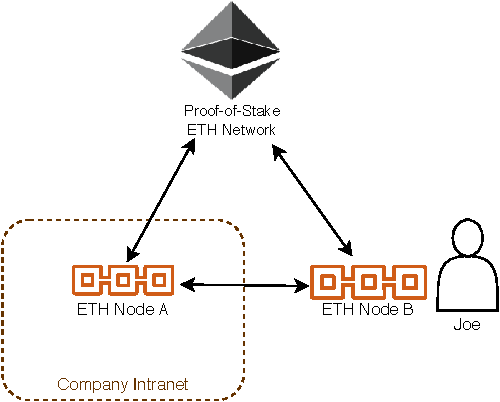
\includegraphics[width=0.7\textwidth]{blockchain_pos}
    \caption{Public Proof-of-Stake network}
    \label{fig:blockchain_pos}
\end{figure}
\begin{figure}[h]
    \centering
    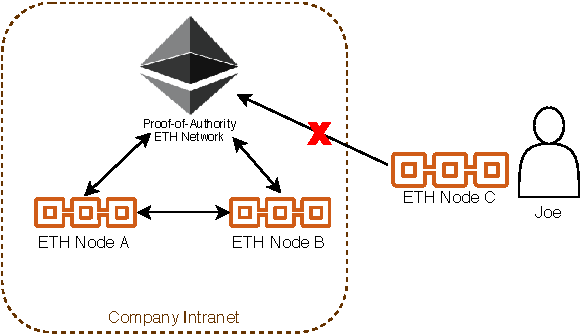
\includegraphics[width=0.75\textwidth]{blockchain_poa}
    \caption{Private Proof-of-Authority network}
    \label{fig:blockchain_poa}
\end{figure}

Figures \ref{fig:blockchain_pos} \& \ref{fig:blockchain_poa} illustrate those differences. In the first example, the company has complete control over its blockchain network, and nobody from the outside can read it or add new blocks. Even though Joe has configured his own node, he will not be able to connect to it. In the second example, the company is connecting to the public node, to which Joe - and anyone else - can also connect to read or submit new blocks.

Let us first look at Proof-of-Stake. This includes all benefits coming from blockchain architecture.  That is, the entire layer is decentralised, meaning that hardware failure will not cause data loss, as every participant will be holding a copy. This ensures a pure 100\% uptime of the data layer. Moreover, all transactions are transparent and immutable. Nobody can deny submitting it or alter the past by removing some blocks from the chain (which is not even possible, to begin with) - perhaps this would be the most beneficial for the authorities and law enforcement organisations, which no longer have to trust data provided by the company, as they can host their own node and read stored data.

\subsection{Comparison with State-of-the-Art}
Both IoT and Blockchain are still developing technologies, which only recently gained traction in the industry. The lack of a similar solution forced me to look beyond the original scope of the project and investigate papers which were also combining those two concepts. Because of that, state-of-the-art comparison involves only the un-changed MQTT Broker. I was satisfied to see only minor increase, while providing the extra security capabilities.
\section{Reflection}
This section will reflect back on the challenges that I faced when working on this project. I will also outline things that went exceptionally well and things that did not go as planned.
\subsection{Achievements}
Before deciding to work on this particular topic, I did not know MQTT or blockchain. I only briefly heard about such technologies, but never had a chance to apply them in any of my projects. The majority of time working on this dissertation was spent on background research and learning how to bring up my own Ethereum network, research industry trends and conducting a thorough evaluation to assess my solution.

I am also happy to say that I successfully followed my original project plan, only with minor deviations. At no point I was facing pressure or closing on deadlines, always leaving an extra week or two as a buffer in case things did not go as expected.

Writing such lengthy documentation was also always a challenge for me, so I am very proud that I was able to stay persistent and finalise this project, gaining valuable research experience.

\subsection{Difficulties \& Lessons Learnt}
When starting to plan this project at the end of the last year, I never anticipated that I would have to conduct it in circumstances of a worldwide lockdown. I have to admit, working on my project entirely remotely has been a big challenge which made me appreciate face-to-face teaching \& guidance even more. As much as my online meetings were going smoothly and without problems, I started to miss the whiteboarding in my supervisor's office - which was invaluable during brainstorming.

As I planned my risk management when writing the project plan, I didn't take global pandemic into account - and I don't think that anyone did. With remote work, I lost the benefit of networking with my peers and discussing our ideas, which provided an immense help before. We were able to overcome this challenge by organising a weekly remote meetup through videoconferencing to carry on, as we knew that the help that we can offer each other is invaluable.

I also learned to always ask for help if faced with a roadblock for an extended time. For example, at one point, I encountered a problem where my software was no longer capable of handling concurrent clients. I spent roughly 2 days dissecting my code line by line, to determine the root cause and eventually pinpointed it to the fact that the Client ID field needs to be unique for the broker to respond. When discussed it with one of my co-supervisors, I learned that he also faced a similar problem in the past and also got stuck for a couple of days. If I approached him earlier, I could have saved those two days.

Several technical challenges also came up, that I either had to omit from the final implementation or think about a workaround. One of the examples being the sheer cost of operating applications on a distributed platform. It is incredibly easy to start exhausting the resources (and thus bumping the price) exponentially, so I had to think about limiting potential writes to a minimum. That's how the caching and crafting data models came to life, as I started to become concious of available resources. Another example is TLS, which almost doubled the response times. I learned that sometimes it might be more desirable to decide against TLS in favour of plain TCP in order to have a more responsive solution.

\section{Future Work}
This section will outline the possible future for FlyTrap and how it could be brought forward with further enhancements to the provided security.
\subsection{Testing TLS}
Following up from the evaluation chapter, we observed a significantly increased performance loss when proxying TLS connections from Client towards FlyTrap and then from FlyTrap to MQTT Broker. Further testing could be needed to determine whether the impact is more significant on \mbox{Client<->FlyTrap} or FlyTrap<->Broker side and provide appropriate guidance on how to provide the best possible performance.

For example, for situations where both FlyTrap and MQTT Broker are located on the same network, it would be wasteful to encrypt packets flowing between FlyTrap and Broker, as man-in-the-middle attacks would not be possible, since all traffic occurs on loopback network device\footnote{Also known as localhost, i.e. inter-process communication through TCP.}. It would be interesting to see whether enabling TLS only on the first part of the journey provides any significant gains.

Furthermore, alternative methods of encrypting TCP packets should be explored. This project uses the standard TLS session with all settings left at default, so tests involving different cypher suites and different key-exchange algorithms would be beneficial.
\subsection{WebSockets}
The most recent versions of popular MQTT Brokers (such as Mosquitto) introduced support for WebSockets - with many of the testing online brokers already offering support, e.g. HiveMQ WebSocket-based broker can be accessed under broker.hivemq.com:8000. WebSocket \cite{fette2011websocket} is built on top of HTTP layer, meaning that all traffic flows through a single port. It is no longer necessary to utilise multiple ports to send concurrent messages.

\begin{figure}[h]
    \centering
    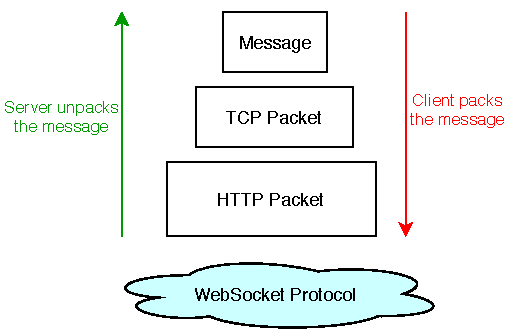
\includegraphics[width=0.7\textwidth]{websockets}
    \caption{Overview of WebSocket protocol}
    \label{fig:websockets}
\end{figure}

Figure \ref{fig:websockets} demonstrates how messages are encapsulated by the client and then unpacked by the server. The most apparent benefit is the increased number of possible proxy connections. FlyTrap currently is tied to the maximum of 65535, which is the maximum number of ports on Linux. Additionally, many firewalls forbid outgoing and incoming connections from non-standard ports. Whenever a new proxy connection is initiated, FlyTrap opens a new ephemeral port, which could otherwise be blocked.

At the moment, the framework operates solely on the TCP layer, sending raw TCP/TLS packets. By adding support for the WebSocket protocol, the limit of maximum concurrent connections could be increased, and by limiting it to a single port (for example, 80), it could become more accessible to devices behind strict firewalls.
\subsection{Device Authenticity}
FlyTrap currently relies only on authentication through a signature containing the public key, signed by the corresponding private key. While it works perfectly fine for the purposes of this project and provides a reasonable protection barrier from attackers, it does not take into consideration situations where the IoT device containing the private key/signature gets stolen, and its data becomes compromised. At this point, the attacker could calculate their own signatures and start making requests against FlyTrap. IoT devices are often neglected when it comes to physical security - they are often placed in public spaces, where anyone could potentially remove it. Normally, it is not a concern, as they are not targeted due to their low cost, but by containing secret data (and signature / private key could be considered secret), it might cause them to become a target.

This problem fell out of scope for this project, and thus it was not considered when designing the system. To tackle this, one might want to introduce methods of verifying the authenticity of connecting devices. In 2012 Apple filed a patent with the United States Patent and Trademark Office \cite{omernick2012systems} offering a solution for this problem. In the future, ideally, FlyTrap should be enhanced by a similar solution, such that it would be able to identify whether the connecting device is a genuine IoT sensor or an attacker connecting from a laptop.

\section{Conclusion}
Through my work in this project, I have shown how Ethereum and MQTT can be combined to provide an efficient Authentication and Accountability framework for MQTT brokers by utilising decentralised blockchain as a data layer. This solution provides a novel set of features such as brute force attack protection, data access monetisation (by collecting payments in a form of cryptocurrency) or a user-friendly front-end to browse the past transactions in order to answer common GDPR questions. The evaluation also proved that the performance impact is acceptable with regards to the gained features. Due to the complex set of dependencies, it is currently aimed at business that are already using blockchain and MQTT, since for them the setup overhead would be minimal. But with the increasing popularity with decentralisied solutions and IoT, FlyTrap could also help business looking to switch, as all needed components (such as MQTT client, front-end or Blockchain CLI) are provided as part of the solution. FlyTrap also has an exciting collection of future work suggestions, which might make it even more accessible and attractive to the potential customers..
